\documentclass[10pt,twocolumn,letterpaper]{article}

\usepackage{iccv}
\usepackage{times}
\usepackage{epsfig}
\usepackage{graphicx}
\usepackage{amsmath}
\usepackage{amssymb}
\usepackage{subcaption}

% Include other packages here, before hyperref.

% If you comment hyperref and then uncomment it, you should delete
% egpaper.aux before re-running latex.  (Or just hit 'q' on the first latex
% run, let it finish, and you should be clear).
\usepackage[breaklinks=true,bookmarks=false]{hyperref}

\iccvfinalcopy % *** Uncomment this line for the final submission

\def\iccvPaperID{****} % *** Enter the ICCV Paper ID here
\def\httilde{\mbox{\tt\raisebox{-.5ex}{\symbol{126}}}}

% Pages are numbered in submission mode, and unnumbered in camera-ready
%\ificcvfinal\pagestyle{empty}\fi
\setcounter{page}{4321}
\begin{document}

%%%%%%%%% TITLE
\title{Multispectral Texture characterization: Application to Mitotic Count in Breast Cancer Histopathology}

\author{Humayun Irshad, Ludovic Roux\\
	University Joseph Fourier Grenoble \\ France\\
	{\tt\small {humayun.irshad, ludvoic.roux}@ipal.cnrs.fr} \\
	\and 
	Alexandre Gouallard\\
	Institution2\\ First line of institution2 address\\
	{\tt\small secondauthor@i2.org} \\
	\and
	Daniel Racoceanu\\
	University Pierre and Marie Curie \\ France\\
	{\tt\small daniel.racoceanu@upmc.fr}
}

\maketitle
%\thispagestyle{empty}

%%%%%%%%% ABSTRACT
\begin{abstract}
Accurate counting of mitosis in breast cancer histopathology plays a critical role in the grading process. Manual counting of mitosis is tedious and subject to considerable inter- and intra-reader variations. We found that the state-of-the-art methods have not significant accuracy on multispectral imaging in histopathology. This study aims at improving the accuracy of mitosis detection by selecting the multispectral spatial features including intensity and textures having mitosis discrimination from other objects. The proposed framework includes comprehensive analysis of spectral bands and z-stack focal planes and selection of multispectral spatial features and a study on candidate detection in different spectral bands. The proposed framework has been evaluated on MITOS Multispectral dataset. The proposed framework achieved $--\%$ detection rate, $--\%$ precision and $--\%$ F-Measure. In future work, we plan to apply multipsectral and multiscale spatial features analysis for mitosis detection.
\end{abstract}

%%%%%%%%% BODY TEXT
\section{Introduction}
Breast cancer (BC) is the most commonly diagnosed cancer after skin cancers, and the second leading cause of cancer death, following lung cancer among U.S. women \cite{jiemin2013}. In 2012, an estimated 226870 new cases of invasive BC and 39,510 BC deaths in women are reported in U.S. In addition, BC incidence and mortality rates have been increasing rapidly in economically less developed countries. According to World Health Organization, the reference process for breast cancer prognosis is histologic grading that combine tubule formation, nuclei atypia and mitotic counts \cite{bloom1957, elston1993}. This assessment of tissue sample is synthesized into a diagnosis that would help the clinician determine the best course of therapy. We found several CAD systems for tubule formation \cite{petushi2006, naik2008} and nuclei atypia \cite{cosatto2008, dalle2009, chaudhury2011, dundar2011}, but only few mitotic counts (MC) \cite{irshad2013a, irshad2013b}. One of the most difficult fields in histopathology imagery is spatial analysis, more specifically automated nuclei detection and classification \cite{fuchs2011}. The objective of nuclei classification is assign label to different type of nuclei as normal, cancer, mitotic, apoptosis, lymphocytes etc that in particular, a challenging problem to address in histopathology. In addition, quantitative characterization is important not only for clinical applications (e.g., to reduce/eliminate inter- and intra-observer variation in diagnosis) but also for research applications (e.g., to understand the biological mechanisms of the disease process \cite{gurcan2009}.
 
In histopathology, H\&E is a well established staining technique that exploits intensity of stains in the tissue images to quantify the nuclei and other structures related to cancer developments. Image processing techniques in this context are devoted to the accurate and objective quantification and localization of such activity in specific regions of the tissue such as cytoplasm, membranes and nuclei. From the chromatic viewpoint, nuclear regions are characterized by non-uniform stain intensity and color, thus preventing a trivial classification based on color separation. In addition, the superposition of tissue layers as well as the diffusion of the dyes on the tissue surface may bring the stains to contaminate the background or other cellular regions which are different from their specific target. Recent work \cite{khan2012b, irshad2013a, irshad2013b} show great potential for CAD of histopathological datasets for breast cancer diagnosis.

In medical image analysis particularly pathology, computer aided detection/diagnosis (CAD) systems are getting popular for clinical purposes (medical procedures seeking to divulge, diagnose or examine disease) and medical science (including the study of body anatomy). CAD systems are extensively used in the detection and differential diagnosis of many different types of abnormalities in medical images obtained using different imaging modalities. Medical image analysis in cytology domains have been major research fields for several decades and numerous systems \cite{ wolberg1993, stewart1998, cibas2009, plissiti2013, gong2013} and software platforms
\footnote{ImageJ, http://rsb.info.nih.gov/ij/}$^,$
\footnote{Mirada Medical, http://www.mirada-medical.com/}$^,$
\footnote{Cyres Cytology, http://www.cyres.co.uk/cytology.php}$^,$
\footnote{PATHOS-WEB, http://pathos-web.sourceforge.net/}
 have been developed for these domains. The application of these systems to histopathology is complicated due to radically different imaging modalities and image characteristics. In case of histology images, cellular structure and function is studied while in histology, whole tissue having cells and architecture like gland formation are studied.
 
Multispectral imaging (MSI) retrieves spectrally resolved information of an image scene at specific frequencies across the electromagnetic spectrum. MSI captures images with accurate spectral content correlated with spatial information and reveals the chemical and anatomic features of histopathology \cite{levenson2006b, levenson2008}. This is because it provides option to biologists and pathologists to see beyond the RGB image planes that they are accustomed to. Recent publications \cite{fernandez2005, levenson2006, wu2012, khelifi2012} have begun to explore the use of extra information contained in such spectral data. Specifically, there have been comparisons of spectral unmixing algorithms (to separate constituent dyes) which demonstrate the advantage of multispectral data \cite{levenson2003, gentry1999}. The added benefit of MSI for analysis of routine H\&E histopathology imagery, however, is still largely unknown, although some promising results are presented in \cite{roula2003, fernandez2005, khelifi2012, wu2012}.

While nuclei segmentation and classification using MSI in histopathology is new area of research, many researchers used single band of MSI for segmentation of tissue and nuclear region \cite{boucheron2007, wu2009, masood2009} and few used all or selected bands \cite{fernandez2005, khelifi2012}. As far as we know, there is no existing study of the advantage of MSI for automation of mitotic counts in breast cancer histopathology. We proposed here to extend the already successful work of \cite{irshad2013b} to automation of MC in MSI.

The reminder of the paper is organized as follows. Section~\ref{sec:previous} reviews the state-of-the-art multispecttral methods, particularly in object or region detection in histopathology, related to this research work. Section~\ref{sec:framework} describes the proposed framework for mitotic figure detection. Experiment and results are presented in section~\ref{sec:results}. Finally, the concluding remarks with future work are given in section~\ref{sec:conclusion}.

%-------------------------------------------------------------------------
\section{Literature Review}
\label{sec:previous}

The main idea of extracting texture from MSI is the use of combined spectral and spatial information for discrimination of region or objects. We found few methods in the MSI literature for texture characterization of histopathological images. Some of them employed single band of MSI and other used multiple selected bands of MSI. Fernandez et al. \cite{fernandez2005} coupled high-throughput Fourier transform infra-red (FTIR) spectroscopic imaging of tissue microarrays with statistical pattern recognition of spectra indicative of endogenous molecular composition and demonstrate histopathologic characterization of prostatic tissue. They explicitly defined metrics to consist of spectral features that have a physical significance related to tissue biochemistry and facilitated the measurement of cell types. The approach in \cite{woolfe2006} used hyperspectral images of colon biopsy slides whereby the classification algorithm was based on spectral analysis to discriminate between normal and cancerous biopsies of the colon tissue. In this study of hyper-spectral cancer analysis, they used Laplacian eigenmaps to take into account the non-linear geometry in the design of learning algorithms and evaluated two approaches for spectral feature selection: Haar wavelet packet best bases (active sensing) and random projections.

Masood et al. \cite{masood2009} proposed a colon biopsy classification method based on spatial analysis of hyperspectral image data from colon biopsy samples. Initially, using circular local binary pattern algorithm, spatial analysis of patterns are represented by a feature vector in selected spectral band. Later, classification is achieved using subspace projection methods like principal component analysis, linear component analysis and support vector machine. Boucheron et al. \cite{boucheron2007} presented an analysis of the utility of multispectral versus standard RGB imagery for pixel level classification of nuclei in H\&E stained histopathological images. 

Khelifi et al. \cite{khelifi2012} proposed a spatial and spectral gray level dependence method in order to extend the concept of gray level co-occurrence matrix by assuming the presence of texture joint information between spectral bands. Malon et al. \cite{malon2013} demonstrated a segmentation based features with convolutional neural networks using additional focal planes and spectral bands for identification of mitotic nuclei in breast cancer histopathology and achieved best classification accuracy (F-measure = 59\%) on multispectral dataset during ICPR context 2013 \cite{roux2013}.

Recently, Wu et al. \cite{wu2012} proposed a multilayer conditional random field model using a combination of low-level cues and high-level contextual information for nuclei separation in high dimensional data set obtained through spectral microscopy. In this approach, the multilayer contextual information was extracted by an unsupervised topic discovery process from spectral images of microscopic specimen, which efficiently helps to suppress segmentation errors caused by intensity inhomogeneity and variable chromatin texture.

In the proposed methodology, we address limitation of the shortcomings in previous works, including (1) comprehensive analysis of multispectral spatial feature vector in all bands rather than single band \cite{masood2009,wu2009,wu2012} and (2) combining spatial feature with multispectral spatial feature vector in order to discriminate mitotic figures from other nuclei and microscopic objects. The main novel contributions of proposed work are: (1) a multispectral spatial and morphology feature vector computation which inherit discriminant information from other nuclei and (2) an projection features from multispectral features vector for classification of mitotic figures in breast cancer histopathological images.

%------------------------------------------------------------------------
\section{Proposed Framework}
\label{sec:framework}
\subsection{Dataset}

We evaluated the proposed framework on multispectral MITOS dataset \cite{mITOS2012}, a freely available mitosis dataset. The data set is made up of 50 high power fields (HPF) coming from five different slides scanned at 40X magnification using a 10 bands multispectral microscope. There are 10 HPFs per slide and each HPF has a size of $512\times512\mu\text{m}^2$ (that is an area of $0.262mm^2$). The spectral bands are all in the visible spectrum. In addition, for each spectral band, the digitization has been performed at 17 different focus planes (17 layers Z-stack), each plane being separated from the other by 500 nm. For one HPF, there are 170 gray scale images (10 spectral bands and 17 layers Z-stack for each spectral band). These 50 HPFs contain a total 322 mitotic cells. The training data set consists of 35 HPFs containing 224 mitotic cells and evaluation data set consists of 15 HPFs containing 98 mitotic cells \cite{roux2013}. Figure \ref{fig:spectral_bands} shows the spectral coverage of each of the 10~spectral bands of the multispectral microscope.
\begin{figure}[t]
	\centering
	\begin{subfigure}[b]{0.5\textwidth}
		\centering
		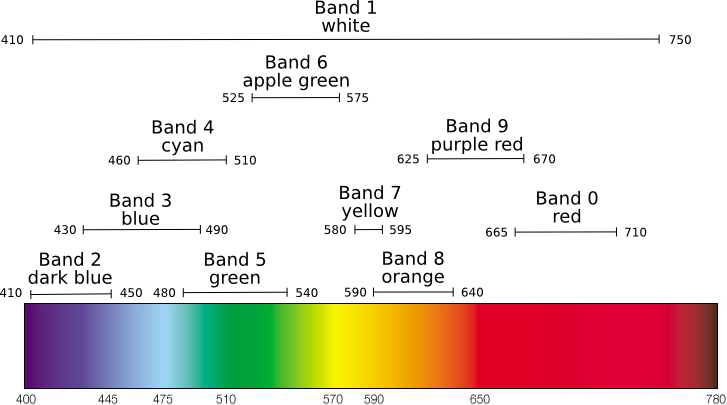
\includegraphics[width=\textwidth]{img/spectral_bands.png}
	\end{subfigure}
	\begin{subfigure}[b]{0.11\textwidth}
		\centering
		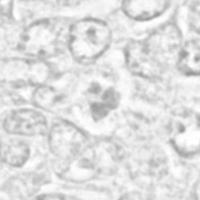
\includegraphics[width=\textwidth]{img/M03_00a_0010_m1.png}
		\caption*{Band 0}
	\end{subfigure}
	\begin{subfigure}[b]{0.11\textwidth}
		\centering
		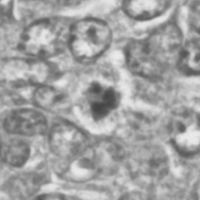
\includegraphics[width=\textwidth]{img/M03_00a_0107_m1.png}
		\caption*{Band 1}
	\end{subfigure}
	\begin{subfigure}[b]{0.11\textwidth}
		\centering
		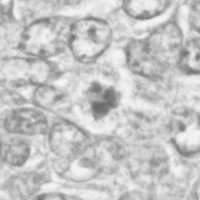
\includegraphics[width=\textwidth]{img/M03_00a_0209_m1.png}
		\caption*{Band 2}
	\end{subfigure}
	\begin{subfigure}[b]{0.11\textwidth}
		\centering
		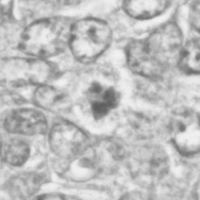
\includegraphics[width=\textwidth]{img/M03_00a_0308_m1.png}
		\caption*{Band 3}
	\end{subfigure}
	\begin{subfigure}[b]{0.11\textwidth}
		\centering
		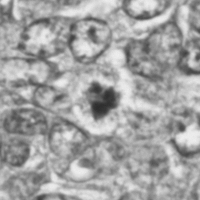
\includegraphics[width=\textwidth]{img/M03_00a_0406_m1.png}
		\caption*{Band 4}
	\end{subfigure}
	\begin{subfigure}[b]{0.11\textwidth}
		\centering
		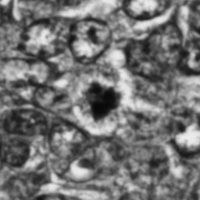
\includegraphics[width=\textwidth]{img/M03_00a_0506_m1.png}
		\caption*{Band 5}
	\end{subfigure}
	\begin{subfigure}[b]{0.11\textwidth}
		\centering
		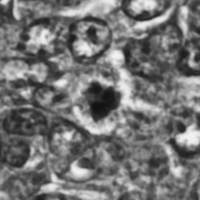
\includegraphics[width=\textwidth]{img/M03_00a_0606_m1.png}
		\caption*{Band 6}
	\end{subfigure}
	\begin{subfigure}[b]{0.11\textwidth}
		\centering
		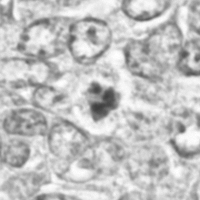
\includegraphics[width=\textwidth]{img/M03_00a_0706_m1.png}
		\caption*{Band 7}
	\end{subfigure}
	\begin{subfigure}[b]{0.11\textwidth}
		\centering
		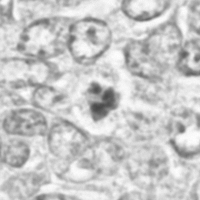
\includegraphics[width=\textwidth]{img/M03_00a_0807_m1.png}
		\caption*{Band 8}
	\end{subfigure}
	\begin{subfigure}[b]{0.11\textwidth}
		\centering
		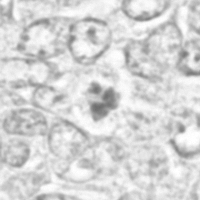
\includegraphics[width=\textwidth]{img/M03_00a_0908_m1.png}
		\caption*{Band 9}
	\end{subfigure}
	\caption{Spectral bands of the multispectral microscope and examples for each band.}
	\label{fig:spectral_bands}	
\end{figure}

\subsection{Proposed Framework}
In this paper, we propose a framework for MC based on spatial analysis of MSI in breast cancer histopathology as shown in \ref{fig:framework}. Initially, a z-stack plane is selected based on gradient and band is selected based on histogram analysis. Then, candidates for mitotic figures  are computed on selected band and z-stack plane. A multispectral feature vector is computed for all detected candidates including intensity and texture features in all bands of multispectral images. In addition, using segmented regions of detected candidates, morphological features are also computed. A feature selection algorithm is employed on this multispectral features vector to save the computation cost and to discard any redundancy in the data in order to improve classification accuracy. Classification is achieved using support vector machine (SVM), Bayesian network (BN) as well as decision tree (DT). A side advantage of performing the spatial analysis on a multiple band is to investigate whether improvement in accuracy can be achieved with carefully selected multispectral features to those methods \cite{masood2009,wu2009,wu2012} which use single band data.
\begin{figure*}
	\centering
	\includegraphics[width=\textwidth]{diagrams/framework.jpg}
	\caption{Proposed Framework.}
	\label{fig:framework}
\end{figure*}

\begin{figure}[b]
	\centering
	\begin{subfigure}[b]{0.22\textwidth}
		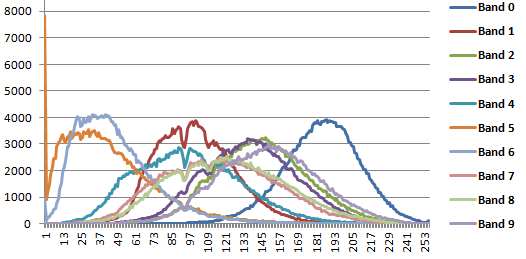
\includegraphics[width=\textwidth]{diagrams/AllBandsHistrogramActual.png}
		\caption*{Mitotic region histogram}
	\end{subfigure}
	\begin{subfigure}[b]{0.22\textwidth}
		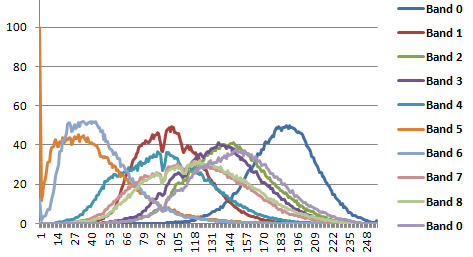
\includegraphics[width=\textwidth]{diagrams/AllBandsHistrogram.png}
		\caption*{Band 0 Histogram}
	\end{subfigure}
	\caption{Histogram analysis of mitotic and background regions in 10 spectral bands.}
	\label{fig:bands_histogram}	
\end{figure}

\subsubsection{Candidate Detection}
Initially, we perform gradient analysis on all the focus planes and select focus plane 10 that is having averagely maximum gradient value. Using selected focus plane, we compute the spectral responses of mitotic nuclei and background regions for all the available 10 spectral bands as represents in \ref{fig:bands_histogram}(a) while responses of mitotic and non mitotic nuclei are presented in \ref{fig:bands_histogram}(b). The peak of the mitotic and non-mitotic nuclei is almost similar but mitotic and mitotic nuclei have different peaks than background regions. It can be said that multispectral data is able to discriminate between different tissue parts but spectral response of mitotic and non-mitotic nuclei is not distinguishable. This motivate us to perform spatial analysis on multispectral data for achieving reasonable classification nuclei into mitotic and non-mitotic nuclei. Using selected focus plane and spectral band, we perform binary thresholding followed by morphological processing to eliminate small regions and fill holes and later select the candidates by filtering based on minimum size ($37\mu\text{m}$ i.e., 200 pixels) and maximum size ($1000\mu\text{m}$ i.e., 5405 pixels ) of mitotic nuclei while keeping the number of of candidates to classify as low as possible. 

\subsubsection{Multispectral Features Computation}
Instead of single band as \cite{boucheron2007, masood2009, wu2009, wu2012}, we compute multispectral spatial feature vectors having intensity and textural features. In addition, we also include morphological features ( such as area, roundness, elongation, perimeter and equivalent spherical perimeter) that are computed from regions segmented during candidate detection. The morphological features reflect the phenotype information of mitotic nuclei. Utilizing spatial information in multispectral bands, we compute five intensity based features including mean, median, variance, kurtosis and skewness for candidate. This results in 50 multispectral intensity based features. Haralick co-occurrence (HC) \cite{haralick1973} and run-length (RL) \cite{galloway1975} features are computed with 1 displacement vector in four direction $(0^o, 45^o, 90^o, 135^o)$ for all the spectral bands as \cite{irshad2013b}. These multispectral textural features are rotationally invariant. So by making average in all four directions, eight HC and ten RL features are computed for each candidate in single spectral band. The resulted multispectral textural features vector consists of 80 HC features and 100 RL features for each candidates. The final multispectral spatial features vector contains 235 features for each candidate. 

\subsubsection{Feature Selection and Classification}
Conceptually, a large number of descriptive features are highly desirable for classification of object as mitosis or non-mitosis. However, when use all computed features (i.e. 235 features) for classification of candidate as mitosis or non-mitosis, the classification performance is poor. Some features are irrelevant for classification and some features are redundant that represents duplication of features and does not provide additional class discriminatory information, degrading the classification performance. Later, we use consistency subset evaluation method~\cite{liu96} to select a subset of features that maximize the consistency in the class values. We evaluate the worth of subsets of features by the level of consistency in the class values using the projection of subset of features from training dataset. The consistencies of these subsets are not less than that of the full set of features. At last, we used these subsets in conjunction with a hill climbing search method, augmented with backtracking value 5, which looks for the smallest subset with consistency equal to that of the full set of features. This procedure achieved 86\% reduction in the dimensionality of features set by selecting 20 features. The selected features contained two morphological, intensity and textural features in different spectral bands. The selected features set is used to train different classifier like random forest (RF) classifier, an ensemble classifier consisting of many decision trees, linear SVM (L-SVM) and non-linear SVM (NL-SVM) classifier~\cite{weka12}. Throughout the experiments, the parameters used in RF classifier are MaxDepth = 10 and NumOfTree = 10. We use L2-loss support vector machine for L-SVM classifier with bias = 1, cost = 1 and eps = 0.01. For NL-SVM classifier, we use rbf kernel with degree of kernel = 3, eps = 0.001 and loss = 0.1.

%------------------------------------------------------------------------
\section{Experiments and Results}
\label{sec:results}
\subsection{Experiments}
We evaluate the proposed framework on MITOS multispectral dataset \cite{mITOS2012}, a freely available mitosis dataset. On training and evaluation sets, the candidate detection stage detects 8650 and 4500 candidates, containing 206 and 93 ground-truth (GT) mitosis from a total 224 and 98 GT mitosis, respectively. Therefore, among the entire candidate mitosis there are 5840 and 3920 non mitosis in the training and evaluation sets. The candidate detection stage generates a large number of non-mitosis and misses 18 and 5 GT mitosis from training and evaluation sets, respectively. 
\subsection{Results}

%------------------------------------------------------------------------
\section{Discussion and Conclusion}
\label{sec:conclusion}
An automated mitosis detection framework for breast cancer MSI based on multispectral spatial features vectors has been proposed. Initially, candidate detection is performed in selected spectral and z-stack focal plane. Then, we compute multispectral spatial feature vectors for each candidate, a highly efficient model for capturing texture features for nuclei discrimination. In future work, we plan to use other multispectral feature models to improve the framework accuracy. 
%------------------------------------------------------------------------
{\small
\bibliographystyle{ieee}
\bibliography{egbib}
}
\end{document}
